\section{求解结果}\label{sec:res}

\subsection{最优第二检测点}

取 $S_1$ 为原点、$\theta_1=0^\circ$，求解式~\eqref{eq:opt} 得表~\ref{tab:best}。
最优点落在可行域外缘：距 $S_1$ 约 $1004$ m（可行域外缘上限为 $1005.0$ m），相对示向度方向
偏 $+37.1^\circ$。最坏定位直径 $134.08$ m，相比只做一次测向的 $1800$ m 缩小 $13.4$ 倍。
注意最优点处"到最坏源的距离"为 $999.95$ m，距可测性边界 $1000$ m 只剩 $0.05$ m 余量——
最优解\textbf{恰好顶在}可测性约束上，这不是巧合：基线越长、交会角越大，定位越好，
而"一定听得到"的要求不让基线再长。

\begin{table}[H]
  \centering
  \caption{最优第二检测点及其性能（$S_1=(0,0)$、$\theta_1=0^\circ$）}
  \label{tab:best}
  \begin{tabular}{lc}
    \toprule
    \textbf{量} & \textbf{结果} \\
    \midrule
    $S_2^*$ 坐标                                   & $(801.13,\;604.96)$ m \\
    距 $S_1$ 的距离 $r^*$                          & $1003.89$ m（可行域外缘上限 $1005.0$ m） \\
    相对示向度的方位差 $\varphi^*$                 & $+37.06^\circ$（镜像解 $-37.06^\circ$ 等价） \\
    最坏定位直径 $J^*$                             & $\mathbf{134.083}$ m \\
    最坏情形（源 / 第二次测向误差）                & $d=1500$ m、$\delta_1=\delta_2=+1^\circ$ \\
    源处交会角 $\gamma$ / 第二点距源 $r_2$         & $40.64^\circ$ / $907.24$ m \\
    最优点到最坏源的距离                           & $999.95$ m（$\le1000$ m，余量 $0.05$ m） \\
    对照：只做一次测向的最坏直径                   & $1800$ m \\
    定位精度提升                                   & $\mathbf{13.42}$ 倍 \\
    \bottomrule
  \end{tabular}
\end{table}

\subsection{最坏情形的几何}

表~\ref{tab:best} 的最坏情形为：源位于 $(1499.77,\;26.18)$ m（即 $d=1500$ m、方位偏
$+1^\circ$），第二次测向的名义方向为 $320.36^\circ$、读数再偏 $+1^\circ$ 得
$321.36^\circ$，此时源处交会角 $\gamma=40.64^\circ$。该情形的定位区域是两条 $\pm1^\circ$
边界射线围成的凸四边形，$4$ 个顶点全部落在 $1800$ m 圆域内（未被截断），直径
$134.083$ m——精确构造值与问题一的解析构造值完全一致（相对偏差 $0$）。最坏情形出现的
位置说明：源越远，第二点看到它的方向越接近与第一点平行（$\gamma$ 越小），定位越差；
四个极点中最远那一对（$d=1500$ m、方位 $\pm1^\circ$）就是"最不友好"的源。

\subsection{候选区域}

按 $\eta=10\%$（即 $J\le147.49$ m）得到候选区域如表~\ref{tab:band}：两条关于示向度方向
镜像的窄弧带，径向范围 $947.6\sim1004.5$ m，方位范围 $\theta_1\pm[25^\circ,40^\circ]$，
合计面积 $0.02069$ km$^2$，仅占可行域的 $4.63\%$。阈值收紧时弧带沿外缘进一步变窄：

\begin{table}[H]
  \centering
  \caption{候选区域（$\eta=10\%$ 及更严阈值）}
  \label{tab:band}
  \small
  \setlength{\tabcolsep}{4pt}
  \begin{tabular}{lccccc}
    \toprule
    $\eta$ & \textbf{阈值 $J\le$} & \textbf{极径范围 / m} & \textbf{方位范围} & \textbf{面积 / km$^2$} & \textbf{占可行域} \\
    \midrule
    $10\%$（采用） & $147.49$ m & $947.6\sim1004.5$ & $\theta_1\pm[25^\circ,40^\circ]$ & $0.02069$ & $4.63\%$ \\
    $5\%$          & $140.79$ m & $978\sim1004$     & $\theta_1\pm[28^\circ,40^\circ]$ & $0.00880$ & $1.97\%$ \\
    $2\%$          & $136.76$ m & $993\sim1004$     & $\theta_1\pm[32^\circ,40^\circ]$ & $0.00289$ & $0.65\%$ \\
    \bottomrule
  \end{tabular}
\end{table}

两条弧带的单瓣面积分别为 $0.010344$ km$^2$（严格相等，见 §\ref{sec:algo} 的镜像讨论）。
也就是说：\textbf{在可行域外缘"偏离示向度 $25^\circ\sim40^\circ$"的那两条窄带里任选一点都行}，
取哪一瓣只取决于现场障碍、路径与耗时的偏好（两瓣效果相同）。

\subsection{适合度图}

图~\ref{fig:suit} 是本文的主要成果图：全域视图给出圆域、源不确定集楔形、$1800$ m 圆域外
的不可行区、可测性透镜（可行域）与整个可行域上的适合度填色（颜色越深越适合）；放大视图给出
可行域内的细网格适合度场与等值线（标注对应的最坏直径 $J$）、橙色候选弧带与最优第二检测点
$S_2^*$ 的极坐标标注；右下内嵌图画出最坏那一次的定位四边形与其 $134$ m 直径，直观解释
"为什么要把交会角做到 $40^\circ$"。图中"不可行"区域指的是不满足可测性保证的位置，
而不是不能去的位置——机器狗可以去，但去了无法保证第二次一定测到。

\begin{figure}[H]
  \centering
  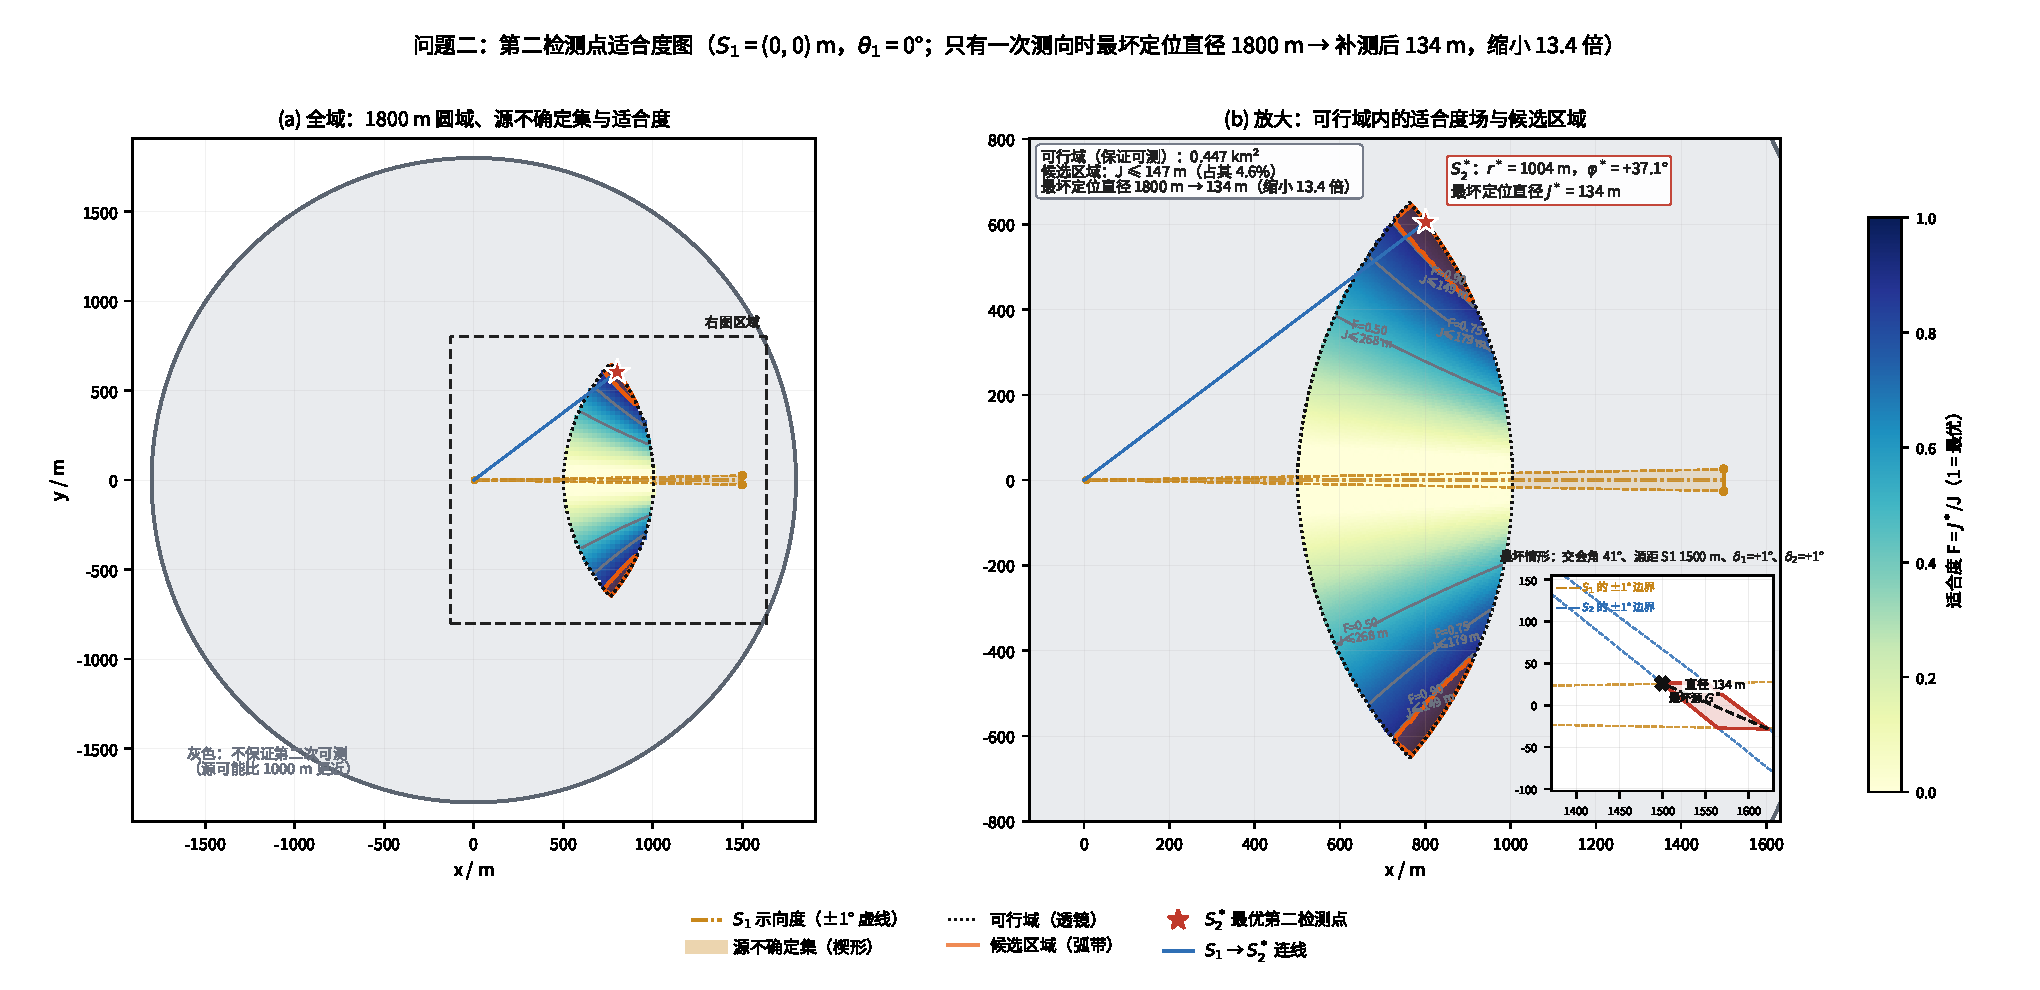
\includegraphics[width=0.98\textwidth]{../figures/t2_suitability.pdf}
  \caption{最优第二检测点与周边区域的适合度场（全域、放大与最坏情形内嵌视图）。}
  \label{fig:suit}
\end{figure}

\subsection{文献判据的对照}

图~\ref{fig:criteria} 把 §\ref{sec:lit} 的四种口径画在一起。左图固定本模型最坏情形的距离
组合（$R_1=1500$ m、$R_2=907$ m），横轴为交会角 $\gamma$，纵轴为定位区域半径（对数坐标）：
精确构造、本文集员闭式、文献 GDOP、文献 CRLB 主半轴与文献几何稀释式五条曲线。可以看到
（i）五条曲线\textbf{走向一致}，都以 $1/\sin\gamma$ 为主导，$\gamma$ 从 $90^\circ$ 降到
$20^\circ$ 时半径放大 $5$ 倍以上；（ii）文献三条曲线明显低于精确构造曲线（约三成），
与表~\ref{tab:criteria} 的数值一致；（iii）本文闭式紧贴精确构造"同口径近似"，在这段
$\gamma$ 区间偏差不到 $10\%$。右图是可行域内 $1276$ 个采样点上"文献 GDOP 判据—本文精确
直径"的双对数散点，点云紧贴对角线（Spearman 秩相关 $0.998$），并标出三个口径各自的最优点。

\begin{figure}[H]
  \centering
  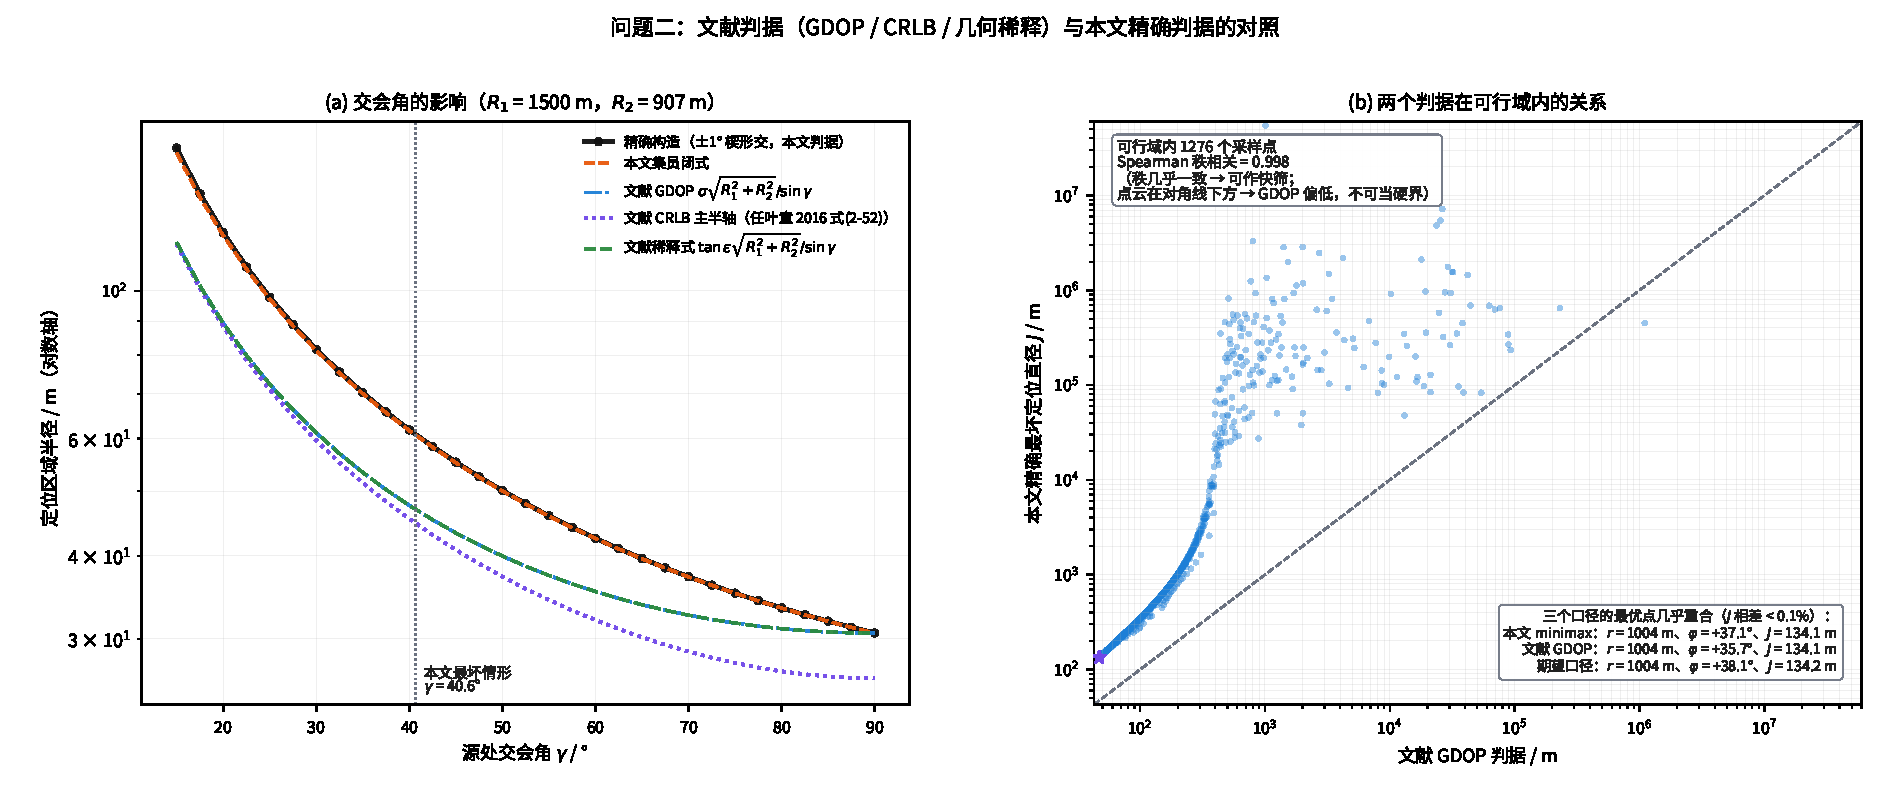
\includegraphics[width=0.98\textwidth]{../figures/t2_criteria.pdf}
  \caption{文献判据与本文判据的对照：(a) 交会角对定位半径的影响；(b) 判据一致性散点。}
  \label{fig:criteria}
\end{figure}

\subsection{准则对照：结论对判据的选择不敏感}

为了回答"换一个判据会不会换一个答案"，本文在完全相同的模型与数据上用三种准则各求一次最
优点，结果列于表~\ref{tab:three}。三个最优点相距不到 $20$ m，最坏直径相差不超过 $0.08\%$，
期望直径相差不超过 $0.2\%$：\textbf{无论按最坏情况、按文献 GDOP 判据、还是按文献常用的期望
精度口径选点，落点都是可行域外缘 $r\approx1004$ m、偏示向度 $36^\circ\sim38^\circ$}。
本文最终采用 minimax 口径，因为清除判据是 $20$ m 硬阈值——需要的是"保证"，不是"平均"。

\begin{table}[H]
  \centering
  \caption{三种准则下的最优点对照（三者都以同一套精确构造与 $1395$ 组合计算）}
  \label{tab:three}
  \small
  \setlength{\tabcolsep}{4pt}
  \begin{tabular}{lccccc}
    \toprule
    \textbf{准则} & $(x,y)$ / m & $r$ / m & $\varphi$ & \textbf{最坏直径 / m} & \textbf{期望直径 / m} \\
    \midrule
    minimax（本文，采用）           & $(801,\;605)$ & $1004$ & $+37.1^\circ$ & $\mathbf{134.08}$ & $56.07$ \\
    文献 GDOP 判据               & $(815,\;586)$ & $1004$ & $+35.7^\circ$ & $134.15$（$+0.05\%$） & $56.18$ \\
    期望精度（Chen 等~\cite{chen2009}）& $(790,\;619)$ & $1004$ & $+38.1^\circ$ & $134.19$（$+0.08\%$） & $\mathbf{56.05}$ \\
    \bottomrule
  \end{tabular}
\end{table}

\subsection{策略的解释}

综合以上结果，第二个检测点的选择策略可以写成三条可以直接执行的规则：

\begin{enumerate}
  \item \textbf{尽量把基线拉长。} 基线越长，源处交会角越大，$1/\sin\gamma$ 越小；但基线受
        可测性限制：源到第二点的距离必须 $\le1000$ m，而源最远可达 $1500$ m，几何上给出
        基线上限 $1005$ m。最优解恰好取在 $1004$ m 处。
  \item \textbf{同时把第二点偏离示向度约 $37^\circ$。} 只拉长基线而方向不变会退化为共线
        （$\gamma\to0$），定位反而变差；偏 $37^\circ$ 既保证"对最远源的交会角最大"，
        又让"对最近源的交会角仍足够大"。
  \item \textbf{两条镜像解等价，任选其一。} 结果关于示向度方向严格镜像对称，现场按障碍与
        路径择优即可。
\end{enumerate}

两个约束同时顶到边界，把最坏交会角锁在约 $41^\circ$——这正是最优点所在处
（若只有基线约束，理论上限是 $\arcsin(1005/1500)=42.1^\circ$，但那时最远源与第二点的距离
会超过 $1000$ m，只能放弃保证）。
